% !TeX program = xelatex
\documentclass{nwputhesis}
\usepackage{gbt7714}
\usepackage{fancyhdr}
\begin{document}

% 生成封面, 使用\maketitle 
% 该封面不同学院要求可能不同,如有需要,请在cls文件中自行修改
\maketitle

\newpage
% 目录
\makecontent
\iffalse
    \makefigcontent
    \maketabcontent
\fi
% 正文
\maketext
\fancyfoot[C]{\thepage}
\pagestyle{fancy}
\section{实习目标}
\subsection{学习方向及目标}
学习现在先进的计算机视觉(Computer Vision)以及图形学与AI结合的模型如Neural Radiance Fields(神经辐射场,简称NeRF),3D Gaussian Splatting(3D高斯溅射,简称3dgs),以及YOLO(全称You Only Look Once),同时理解各个模型的实现原理。
\subsection{期望}
\begin{itemize}
    \item 完成搭建尽可能多的AI模型,配置其环境,并完成训练其预设数据库。
    \item 学习并理解各个模型的实现原理。
    \item 自己制作数据并通过基于AI的三维重建制作模型。
\end{itemize}
\makespace
\section{模型的搭建以及学习}
\subsection{Yolo V5}
\subsubsection{模型简介}
Yolo(You Only Look Once)是一种单阶段目标检测算法,即仅需要 “看” 一次就可以识别出图片中物体的class类别和边界框。Yolov5是由Alexey Bochkovskiy等人在YOLO系列算法的基础上进行改进和优化而开发的,使其性能与精度都得到了极大的提升。
\subsubsection{模型环境配置}
\begin{itemize}
    \item Python = 3.8.19
    \item torch = 2.3
    \item torchvision = 0.18.0
    \item gitpython = 2.40.1
    \item opencv-python = 4.9.0.80
    \item matplotlib = 3.7.5
    \item pandas = 2.0.3
\end{itemize}
模型从\underline{https://github.com/ultralytics/yolov5.git}克隆下来,然后在本地进行配置。

\subsubsection{模型训练}
\indent 模型训练是在\underline{train.py}文件中进行的,训练时可以同时输入data\footnote{文件中包含了训练集和验证集的路径,以及所有的标注种类}、cfg\footnote{文件中包含了模型的参数,如学习率、batch size等}和weight\footnote{文件中包含了预训练模型的权重}文件;或是epochs\footnote{训练的次数}和batch size\footnote{每次训练的图片数量}。
\\
如下图:
\begin{figure}[H]
    \centering
    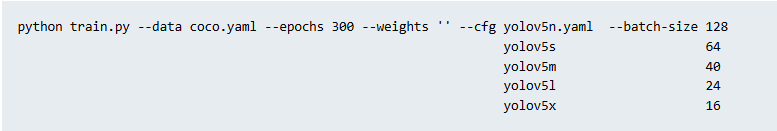
\includegraphics[width=0.8\textwidth]{picture/2.png}
    \caption{YOLOv5目标检测模型的训练命令}
\end{figure}
\subsubsection{测试自己制作的数据集}
从网上找寻了30张宝可梦的图片,然后通过labelImg工具\footnote{LabelImg 是一个开源的图像标注工具,用于创建图像数据集时标记图像中的对象边界框}标注这些图片中比较常见的宝可梦,如皮卡丘、杰尼龟等,然后将这些图片和标注文件放入到一个文件夹中。最后通过YOLOv5模型进行训练,得到了一个可以识别这些宝可梦的模型,因为数据集比较小,所以模型的识别率不是很高。
\\
\indent 训练结果示例:
\begin{figure}[H]
    \centering
    
\includegraphics[width=0.8\textwidth]{picture/3.png}
    \caption{YOLOv5目标检测模型的训练结果}
\end{figure}
\subsubsection{实现原理}
YOLOv5首先会在输入端中将输入图片进行预处理,图像大小调整为模型所需的大小,进行归一化操作,及将像素值缩放到0到1之间。\\
\indent 然后将图片输入到backbone网络\footnote{backbone网络是一个特征提取网络,用于提取图片的特征}中,backbone网络会将图片的特征提取出来,然后将这些特征输入到neck网络\footnote{neck网络是一个特征融合网络,用于将不同层次的特征进行融合}中,neck网络会将不同层次的特征进行融合,然后将这些特征输入到head网络\footnote{head网络是一个预测网络,用于预测图片中的物体}中,head网络会将图片中的物体进行预测,得到物体的类别和边界框。
\\
\indent 下图为YOLOv5的网络结构:
\footnote{CPL:由卷积Conv+批量归一化BN+激活函数Leaky Relu组成,用于在特征提取的过程中增加网络的信息传递能力。CPL通过在不同阶段的特征图之间进行部分连接,使得网络可以更充分地利用低级和高级特征,从而提高模型的性能。}
\footnote{CSP1:由CBL模块、Res uint模块以及卷积层Concat组成。CSP1是CPL的一种变体,它在CPL的基础上引入了跨阶段的残差连接,以进一步增强网络的信息传递能力。CSP1可以有效地减少网络中的计算量,提高模型的效率。}
\footnote{CSP2:不再使用Res unit,由卷积层CBL模块Concat组成。CSP2引入了路径重排的技术,以重新排列网络中的路径,使得前向和后向传播之间的信息流更加平滑和高效。这种路径重排有助于减少网络中的计算量,提高模型的速度和效率。CSP2同样也进行了路径融合(Path Fusion),即在不同路径之间进行信息融合,以使网络可以更充分地利用低级和高级特征。这种路径融合有助于提高模型对目标的检测和识别能力。CSP1也具有类似的路径融合机制。}
\footnote{SPP是一种用于空间金字塔池化的技术,它能够在不同尺度下提取图像的局部特征。SPP在YOLOv5中用于提取特征图的空间信息,从而使得模型可以更好地检测不同尺度和大小的目标。}
\footnote{Focus:对图像进行切片后再Concat}
\footnote{上采样:利用元素复制扩充的方法使得特征图尺寸扩大,例如线性插值。}
\footnote{Concat:张量拼接,会扩充两个张量的维度,实现多尺度特征融合。}
\begin{figure}[H]
    \centering
    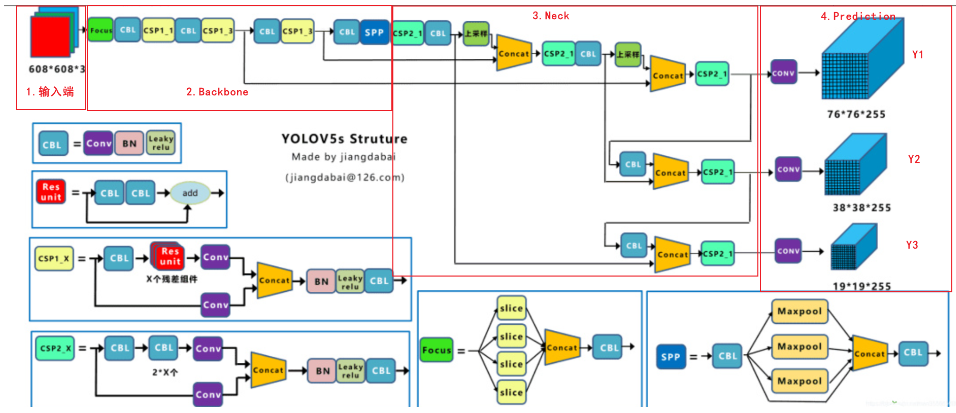
\includegraphics[width=0.8\textwidth]{picture/4.png}
    \caption{YOLOv5的网络结构}
\end{figure}
\makespace
\subsection{NeRF}
\subsubsection{模型简介}
NeRF(Neural Radiance Fields)是一种用于三维重建的深度学习模型,它可以从二维图像中重建出高质量的三维场景。NeRF的核心思想是利用神经网络来建模场景中每个空间点的辐射亮度和密度,从而实现对场景的准确重建。
\subsubsection{模型环境配置}
\noindent 于CUDA 10.2 基础下:
\begin{itemize}
    \item Python = 3.7.1
    \item cudatoolkit = 10.0.130
    \item tensorflow = 1.14.0
    \item numpy = 1.21.5
    \item imageio = 2.193
    \item configargparse = 1.4
\end{itemize}
于CUDA 12.x 基础下:
\begin{itemize}
    \item Python = 3.7.1
\end{itemize}
模型从\underline{https://github.com/bmild/nerf.git}克隆下来,然后在本地进行配置。

\subsubsection{模型训练}
\indent 模型训练是在\underline{run\_nerf.py}文件中进行的,需要同时输入配置文件的的相对路径,配置文件中包含了实验名称(expname),基础目录(basedir),数据集路径(datadir),数据集类型(dataset\_type)采样参数、使用视角方向信息等模型训练和数据配置信息。
\makespace
\section*{致谢}
\begin{center}
    { \blackti \fontsize{16.0600pt}{1.25}致 \, 谢}
\end{center}
\addcontentsline{toc}{section}{致\texorpdfstring{ \, }{} 谢}
\myspace{1}
致谢内容。

% 毕业设计小结
\section*{毕业设计小结}
\makespace
\begin{center}
    { \blackti \fontsize{16.0600pt}{1.25}毕业设计小结}
\end{center}
\addcontentsline{toc}{section}{毕业设计小结}
\myspace{1}
小结内容。

% 附录
\makespace
\section*{附录}
\begin{center}
    { \blackti \fontsize{16.0600pt}{1.25}附 \, 录}
\end{center}
\addcontentsline{toc}{section}{附\texorpdfstring{ \, }{} 录}
\myspace{1}
附录内容。
\end{document}

